\label{game}

This chapter represents a novel game-based methodology for the possible discovery of aircraft optimal escape maneuver against an attacking missile. This discovery could be achieved through a mathematically-correct game of target-attacker where a human player controls the target, trying to evade the missile.  The game is distributed to some ordinary persons (typically young kids) who are asked to play the game and to get the highest scores possible. Best escape maneuvers are collected, analyzed, and optimized, to find the optimal human-based escape maneuver. The game is based on 2D point-mass models for target and attacker and a proportional navigation law for missile guidance. The game is developed using Unity, a free cross-platform game engine. The preliminary results obtained suggest the production of enhanced versions of the game with more desirable outcomes, to utilize collective human-brain capability in producing a new guidance law which could possibly compete with existing ones.

%===============================================================================
\section{Introduction}

Missile avoidance is a very important element of aircraft survivability against attackers in air combat and defense. If the missile guidance law (PN for example) and its parameters (speed, location, etc.) are known, the best avoidance maneuver is the solution of an optimal control problem which can be solved using different optimization techniques such as genetic algorithms (GA) or particle swarm optimization (PSO).  In this work, we try to explore the hypothesis that optimal avoidance strategy can be generated through a completely different approach. A human based approach where humans (most probably kids) are given the problem of missile avoidance in a sort of a game and they are asked to play the game and to get the highest score possible.

In this chapter, we try to benefit from the emergence of novel paradigms for games played by humans versus computers. These paradigms include:

\begin{itemize}
	\item 	\textbf{Competitions} between humans and computers in games of increasing difficulty, including the games of Chess \cite{hsu2002behind}, Arimaa \cite{syed2003arimaa}, Jeapordy! \cite{ferrucci2013watson}, and Go \cite{gelly2011monte}. Typically, the rivalry is between a single human champion (such as Kasparov) against a state-of-the-art computer (such as Deep Blue) limited to a specific domain (such as Chess). The sole purpose of the competition is to decide whether the human or the computer wins more games within the same match.
	
	\item The \textbf{gamification} phenomenon \cite{seaborn2015gamification,dubbels2013gamification,boughzala2016introduction}, which is the use of game design elements in non-game or learning contexts, a trend related to human-computer interactions in the form of serious games, pervasive games, alternate reality games, or playful design.
	
	\item The paradigm of \textbf{games with a purpose} \cite{von2006games,von2008designing,siorpaes2008games,good2011games,jain2008game}, which aims to utilize the billions of hours spent (wasted!) by contemporary humans in playing computer games. This paradigm channels game playing into useful work by directing people playing computer games to simultaneously solve large-scale problems without consciously knowing about this and, hence, without losing the element of fun or entertainment. Many large-scale open problems can be solved using collective human brainpower in this unique way. Examples include language translation, monitoring of security cameras, improving Web search, and text summarization. With the paradigm of games with a purpose, hundreds of millions of people can collaborate on the same problem via the Internet.
	
	\item \textbf{Human Computation} \cite{quinn2011human}, which is the idea of using human brain processing power to perform tasks that computers cannot yet perform or solve problems still intractable for computers, usually in an enjoyable manner. Human Computation is also viewed as systems of computers and large numbers of humans that work together in order to solve problems that could not be solved by either computers or humans alone.
	
	\item \textbf{Crowdsourcing} \cite{brabham2008crowdsourcing}, which is the act of taking a job traditionally performed by a designated agent (an employee) and outsourcing it to a generally large group of people in the form of an open call. Whereas human computation replaces computers with humans, crowdsourcing replaces traditional human workers with members of the human public.
\end{itemize}

This chapter introduces yet another novel paradigm of a game played by humans versus computers. This paradigm resembles that of games with a purpose, but it will neither handle a large-scale open problem nor require a dramatically huge number of human players. The current paradigm might also be viewed as an offshoot of that of human computation, wherein we relax the requirement of dealing with tasks that computers cannot yet perform, and relegate it to handling somewhat sophisticated and complex (but not intractable) tasks. The current paradigm is to solve problems requiring mathematically-elaborate game-theoretic techniques (that already have many automated algorithmic solutions) by requesting a relatively small number of people (~ 50 persons) to play a computer game, constructed to result in a correct solution and, at the same time, is enjoyable. The basic idea is that people will play a game to be entertained, not to solve a problem—no matter how noble and glorious the objective is. The game played constitutes a human-computer competition, but unlike the Kasparov-Deep Blue one, neither the human players are necessarily highly-competent or champions, nor is the computer necessarily of super characteristics. The task encountered herein of designing an online game is much like designing an algorithm. In fact, this game must be proven correct, and its efficiency might be analyzed, so that more efficient versions should always be sought so as to supersede less efficient ones. Instead of using a silicon processor, these “algorithms” run on a processor consisting of the brains of ordinary humans interacting with a computer.


The problem considered herein is an important pursuit-evasion problem that involves two agents, the target (aircraft) and the attacker (missile) \cite{stevens2015aircraft,perh2011study,eklund2012switched,hsueh2014integrated,sun2014guidance}. The attacker missile pursues the target aircraft, and a dynamic or differential game arises in which the target tries to maximize the separation between itself and the attacker, while the attacker tries to minimize this separation. We present a game-based methodology to find the optimal escape maneuver for the target (represented by a human player) against the attacking missile (represented by the computer). The missile pursuit the target according to the 2D guidance law of proportional navigation. The cost function used maximizes the missile acceleration, time to interception and the miss distance. We construct a mathematically-correct game of target-attacker and let many ordinary people play it individually from the target side, and assign a score to every player that is proportional to the cost function. We find the best escape maneuver by collecting and analyzing data of the escape maneuver of the human players. The game is developed using Unity, a free cross-platform game engine.

Since our game is a skill-and-action game, it is characterized by real-time play, and it would definitely benefit of heavy emphasis on graphics and sound and also of the use of joysticks or paddles rather than just a keyboard \cite{crawford1984art}. Moreover, the primary skills demanded of the players of our game are psychomotor skills including hand-eye coordination and fast reaction or response time. The game is somewhat related to combat games, but it is not a combat game per se, since it does not involve a direct mutual violent confrontation between two opponents. The human player, placed in the role of the aircraft, must avoid being captured or hit by the attacking computer-controlled missile, but cannot benefit of the wisdom that retaliatory attack is the best way of evasion or defense.  In fact, the game is a purely defensive one, in the sense that the player never has the opportunity to attack the enemy missile. The game seems somewhat to be a race game since it involves some sort of race between two opponents, but this race is not a straightforward one and it encompasses certain strategic elements.

The present approach can be evaluated as a sort of Reinforcement Learning (RL), a major technique of soft computing for adaptive optimal control of nonlinear systems \cite{liu2009pursuit,sharma2010synergizing,doya2000reinforcement}, where a player takes a long series of actions (moving the aircraft up and down) before receiving the reward (the final score). So, it is hard to decide, mathematically, which of the actions were responsible for the eventual payoff.

In the remainder of this Chapter, we describe the game engine used explain how our game is built. The missile model to be supplied to the computer was earlier described in detail in Section \ref{PNeq}. We also report preliminary results of our new methodology.


\section{Game description and design}

This Section briefly introduces the game engine Unity and explains the first version of our game (henceforth referred to as $Evasion-1$). 
Game design is an artistic process as well as a technical one, and hence its essence is to manage the integration of these two dissimilar processes \cite{crawford1984art}. The purpose of the design is to create outlines of three interdependent structures: the I/O structure, the game structure, and the program structure. The I/O structure constitutes the language for communicating information between the computer and the player. The game structure is a means of figuring out how to distill the goal and topic of the game into a workable system, and identifying some key element or elements around which the game is built. The program structure is the organization of main code, subroutines, interrupts, and data that make up the entire program. All three structures must be created simultaneously, for they must work in harmony. Decisions primarily relating to one structure must be checked for their impacts on the other structures. Once all three structures are made to work in compatibility with one another, it is necessary to evaluate the overall design for the most common design flaws that plague games and to assure that the design satisfies the design goals. The design phase is followed by the programming phase. Programming itself is straining, strenuous and tedious work, requiring attention to detail more than anything else. It might prove to be the hardest of all phases, though its inherent difficulty is somewhat eased by the availability of game engines such as Unity, which is free and simple-to-use beside being able to work on almost any computer and allowing any novice user to download and use its program, and to avoid some of the complex programming techniques through utilizing pre-constructed building blocks.
% The design phase is followed by the programming phase. 
%Programming itself is straining, strenuous and tedious work, requiring careful attention to detail. Its inherent difficulty is somewhat eased by the availability of game engines such as Unity. 

\subsection{Introduction to Unity}

Unity is a cross-platform game engine (Fig. \ref{UnityInterface}), used to develop video games for PC, consoles, mobile devices and websites. It works with the C-sharp programming language, and can be downloaded free of charge from (https://unity3d.com/), which is the official site of its developer (Unity Technologies).


\begin{figure}[H]
	\centering
	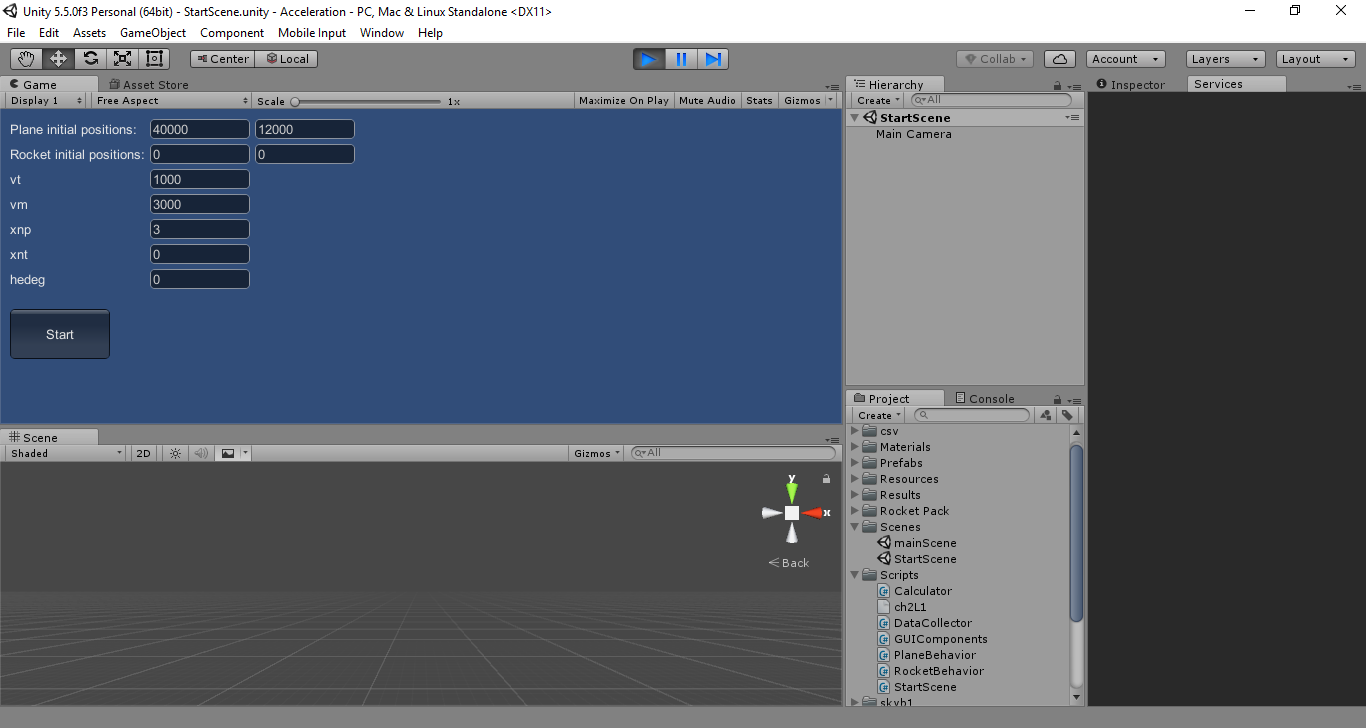
\includegraphics[scale = 0.30]{fig/unityInterface.PNG}
	\caption{Unity game engine interface }
	\label{UnityInterface}
\end{figure}

%===================================================================================

\subsection{Methodology of the game}

Figure \ref{UnityGame} illustrates a typical snapshot or computer screen for Evasion-1, showing the two objects that comprise the game, viz., the plane and the missile. The background has stationary shapes (such as clouds) that set a frame of reference allowing the human player to visually estimate the speeds of the plane and missile. The player controls the acceleration of the target (XNT) using the Up/Down arrows on the keyboard to increase/decrease this acceleration.   Missile motion is computer-controlled according to proportional navigation(in sec. \ref{PNeq}). The game has a few adjustable parameters (see Fig. \ref{UnityInterface}), and hence might be adapted for other pursuit-evasion problems.

 \begin{figure}[H]
 	\centering
 	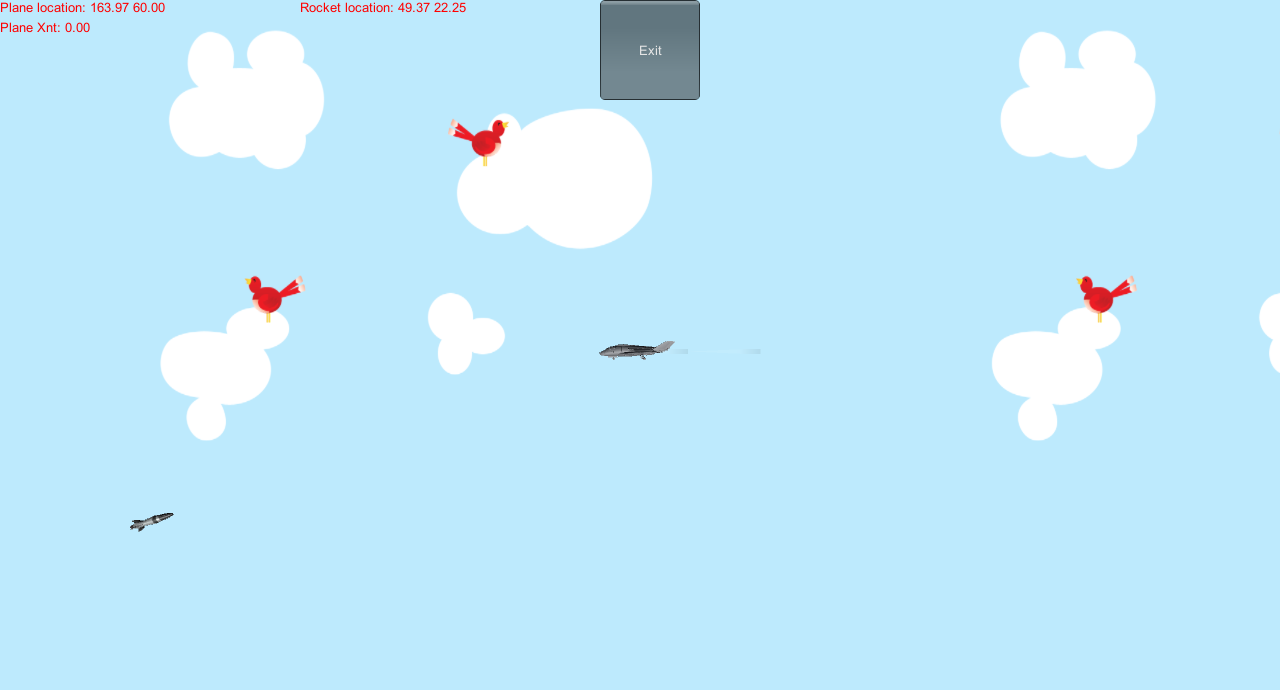
\includegraphics[scale = 0.32]{fig/unityGame.PNG}
 	\caption{Unity game for simulating Target-Attacker engagement}
 	\label{UnityGame}
 \end{figure}
 

Each game consists of two scenes:

\begin{enumerate}
	\item Start or initial scene.
	\item Play scene, updated each frame per second.
\end{enumerate}

In the start scene, there are data fields such as position and velocity, which are destroyed at the end of the scene. Therefore, it is necessary to save all needed information in a file called "player prefs". The play scene consists of several objects (currently three). Each object usually has its own script, which must contain two points:
\begin{itemize}
	\item Start: initialize.
	\item Update: every frame.
\end{itemize} 

The present three objects of the game are:
\begin{enumerate}
	\item \textbf{Plane:} with a script containing some commands to control the plane by increasing and decreasing the target acceleration by the upward and downward arrows, respectively,
	\item \textbf{Missile:} which does not contain a script of its own, since the equations controlling its behavior are within the script of the fictitious "Data collector" object,
	\item \textbf{Object "Data collector":} whose script consists of:
	
	\begin{itemize}
		\item Start
		\begin{enumerate}
			\item initialization of the variables in the equations.
			\item Setting the location of the real objects (plane and missile).
		\end{enumerate}
		\item Update 
		\begin{enumerate}
			\item Getting plane location,
			\item Executing PN equations,
			\item Updating rocket location (according to PN equations),
			\item Updating information to be printed to Excel,
			\item Checking the condition for game termination, and if true, reloading the start scene.
		\end{enumerate}
	\end{itemize}


\end{enumerate} 




%===================================================================================
 
\section{Preliminary ٌٌResults and Analysis}	

Our experience with Evasion-1 demonstrates that the game is working correctly. Figures \ref{trajectory}-\ref{XNC} illustrate some of our preliminary results, obtained by the player with the best score so far. The target acceleration curve in Fig. \ref{XNT} exhibits a Barrel-Roll behavior, an aerial maneuver in which an airplane makes a complete rotation on both its longitudinal and lateral axes, causing it to follow a helical path, approximately maintaining its original direction. This maneuver helps a target to force an attacker to fly out in front, i.e., to overshoot. The results is very encouraging, indeed, since a human player who is definitely unaware of the technicalities of evasion techniques, and who is playing the game just for fun, was remarkably capable of producing an evasion policy, that is considered one of the best in the literature (see, e.g. Zarchan ). The results suggest the production of enhanced versions of the game with more desirable outcomes. Specifically, in our next version (Evasion-2), the plane will no longer be destined to be intercepted by the missile, since we will impose the restriction that the missile has a limited reservoir of fuel that could be drained as a result of clever target maneuver. The ultimate goal is to test human brain capability to work collectively to produce a new guidance law which could possibly compete in accuracy with the existing ones, while surpassing them in the simplicity of the way it is produced. 

 \begin{figure}[H]
	\centering
	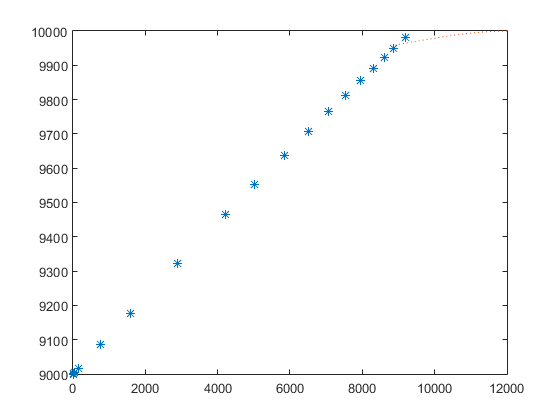
\includegraphics[scale = 0.70]{fig/trajectory.PNG}
	\caption{Target-Attacker 2D trajectory. The target and missile speeds are 3000 m/s,1000 m/s respectively.}
	\label{trajectory}
\end{figure}

 \begin{figure}[H]
	\centering
	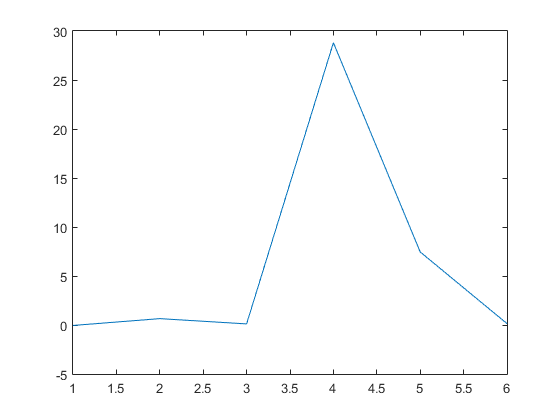
\includegraphics[scale = 0.70]{fig/XNT.PNG}
	\caption{Optimized target acceleration versus time.}
	\label{XNT}
\end{figure}

 \begin{figure}[H]
	\centering
	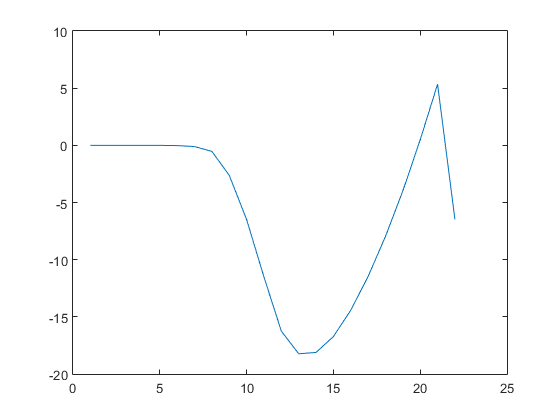
\includegraphics[scale = 0.70]{fig/XNC.PNG}
	\caption{Missile acceleration versus time.}
	\label{XNC}
\end{figure}

\afterpage{\blankpage}
